\chapter{药物代谢动力学}
药物代谢动力学(pharmacokinetics)主要研究内容为两部分:药物的体内过程(吸收、分布、代谢和排泄)和药物在体内随时间变化的速率过程及重要参数。

\section{药物的体内过程}

药物从进入机体至离开机体,可分为四个过程:
\begin{center}
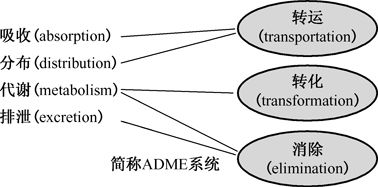
\includegraphics{./images/Image00023.jpg}
\end{center}
\subsection{体内过程的基本规律}
\begin{center}
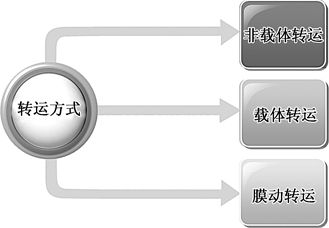
\includegraphics{./images/Image00024.jpg}
\end{center}
(一)非载体转运

被动转运(passive
transport):指药物由浓度高的一侧向浓度低的一侧进行跨膜转运。

特点:①不需要载体;②不消耗能量;③转运时无饱和现象;④无竞争性抑制现象;⑤当膜两侧浓度达到平衡时,转运即保持在动态稳定水平。

1.滤过(水溶扩散)

滤过(filtration)指直径小于膜孔的水溶性的极性或非极性药物,借助膜两侧的流体静压和渗透压差被水携带到低压侧的过程。

胃肠黏膜:胃肠黏膜上皮细胞间的裂隙为4~8A,可滤过100~150道尔顿的物质。

\begin{figure}[!htbp]
 \centering
 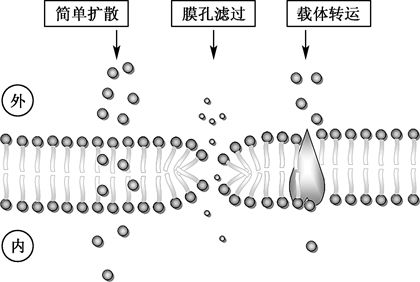
\includegraphics{./images/Image00025.jpg}
 \captionsetup{justification=centering}
 \caption{药物的转运方式}
 \label{fig3-1}
  \end{figure} 

组织中的毛细血管上皮细胞间的裂隙为60~120A,可滤过20000~30000道尔顿的物质,肌肉注射的药物主要通过这种方式吸收。

肾小球滤过:上皮细胞间隙较大,小于60000~70000道尔顿的物质可以滤过。白蛋白分子量为66854道尔顿,是肾小球滤过的一种最小蛋白质,但几乎被近曲小管全部重吸收。当肾小球病变时,白蛋白滤过量超过肾小管重吸收量,则导致尿中白蛋白含量升高,可用于发现早期糖尿病肾病。

2.简单扩散(被动扩散,脂溶扩散)

脂溶性大、极性小(不易离子化)的药物易通过。

通透量(单位时间通透分子数)=(C\textsubscript{1} -C\textsubscript{2}
)×面积×通透系数/厚度

影响跨膜转运的药物理化性质:

(1)分子量。

(2)溶解性:指药物具有的脂溶性和水溶性。

(3)解离性:非解离型药物脂溶性大,易扩散。解离型极性大,脂溶性小,难以扩散。

离子障(ion
trapping)是指非离子型药物可以自由穿透,离子型药物被限制在膜的一侧的现象。

弱酸或弱碱药物的解离(handerson-hasselbalch公式):

以弱酸药物为例:
$$\ce{HA <=>[K_a] H+ + A}$$

10\textsuperscript{pH-pK\textsubscript{a}}
=$\frac{[A^-]}{[HA]}$当pH=pK\textsubscript{a}
时,[HA]=[A\textsuperscript{-} ]

pK\textsubscript{a} 即弱酸性或弱碱性药物在50%解离时的溶液pH值。

当细胞膜两侧pH值不等时,简单扩散的跨膜转运规律如下:弱酸性药物易从酸侧进入碱侧,而弱碱性药物易从碱侧进入酸侧。

当跨膜扩散达到平衡时,弱酸性药物在较碱侧的浓度大于较酸侧,而弱碱性药物在较酸侧的浓度大于较碱侧。

意义:影响药物的吸收、排泄,如:碱化血液和尿液可以使酸性药物(苯巴比妥)加速排泄。

例:丙磺舒的pK\textsubscript{a} =3.4

\begin{figure}[!htbp]
 \centering
 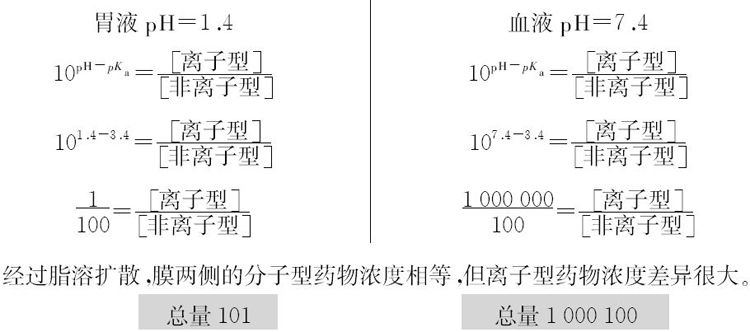
\includegraphics{./images/Image00028.jpg}
 \captionsetup{justification=centering}
 \caption{pH对药物简单扩散的影响}
 \label{fig3-2}
  \end{figure} 

(二)载体转运

载体转运(carrier transport)有主动转运(active
transport)和易化扩散(facilitated
diffusion)两种。共同特点是:①需膜上特异性载体蛋白,有结构特异性;②有饱和性、竞争性。

1.主动转运(active transport)

主动转运的特点:①逆浓度梯度转运;②消耗能量,需ATP,易受代谢因素影响。

2.易化扩散(facilitated diffusion)

易化扩散的特点:①顺着浓度梯度或电化学梯度扩散,转运速度快;②不耗能,不需供应ATP。

(三)膜动转运(cytosis)

1.胞饮(pinocytosis)

\begin{figure}[!htbp]
 \centering
 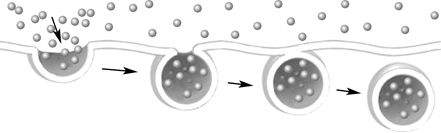
\includegraphics{./images/Image00029.jpg}
 \captionsetup{justification=centering}
 \caption{胞饮}
 \label{fig3-3}
  \end{figure} 

2.胞吐(exocytosis)

\begin{figure}[!htbp]
 \centering
 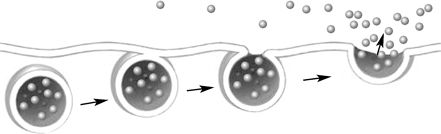
\includegraphics{./images/Image00030.jpg}
 \captionsetup{justification=centering}
 \caption{胞吐}
 \label{fig3-4}
  \end{figure} 

(四)存在形式

\begin{figure}[!htbp]
 \centering
 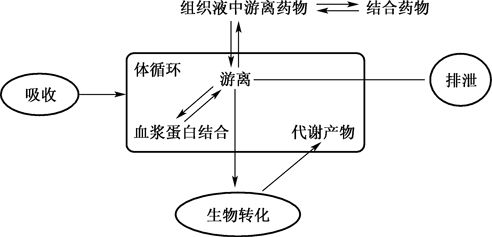
\includegraphics{./images/Image00031.jpg}
 \captionsetup{justification=centering}
 \caption{药物在体内的存在形式}
 \label{fig3-5}
  \end{figure} 

药物在体内通常以游离型和结合型两种方式存在。可以与蛋白结合,如血浆蛋白、组织蛋白,也可以与脂肪、骨骼结合。

\subsection{药物的吸收及影响因素}

(一)吸收

吸收(absorption):指药物从用药部位进入血液循环的过程。

【给药途径】

口服、舌下、直肠、吸入、皮肤、肌注、皮下注射和静脉注射。

【吸收速度】

吸收速度由快至慢依次是:腹腔注射、吸入、舌下、直肠、肌肉注射、皮下注射、口服、皮肤。

1.消化道吸收(enteral absorption)

(1)口腔吸收:口腔黏膜吸收,口腔速溶片,舌下含片。首过消除小。

(2)胃吸收:胃酸影响大。

(3)小肠吸收(口服):面积大,环境偏碱。

胃肠吸收后,都要经过门静脉进入肝,再进入血液循环。首过消除影响大。

(4)直肠吸收:不能口服时,可直肠给药。直肠和结肠的黏膜吸收,2/3无首过消除,可直肠给药(栓剂),首过消除小。

首过消除:口服药物在通过胃、肠黏膜及肝脏时被部分灭活,使进入体循环的药量减少的现象。例如,某药被肠黏膜代谢30%,肝脏代谢45%,进入体循环的药物只有15%(图\ref{fig3-6})。

\begin{figure}[!htbp]
 \centering
 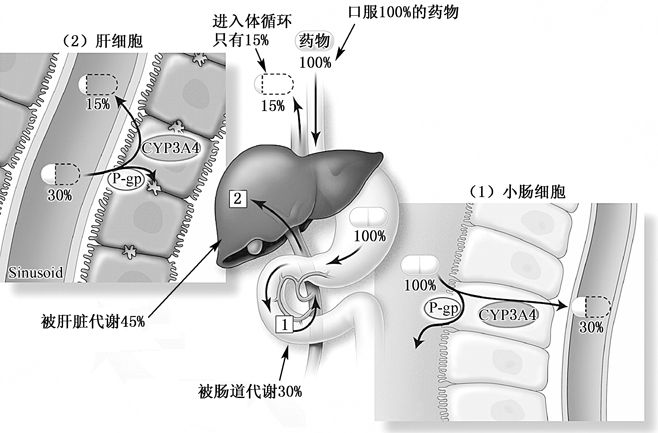
\includegraphics{./images/Image00032.jpg}
 \captionsetup{justification=centering}
 \caption{首过消除}
 \label{fig3-6}
  \end{figure} 

2.注射(injection)

(1)静脉注射给药(intravenous):直接将药物注入血管。

(2)肌肉注射和皮下注射(intramuscular and subcutaneous
injection):主要以滤过和被动扩散的方式吸收,快而全。

通常肌肉注射吸收快于皮下注射,循环障碍时应静注。此时,肌肉或皮下注射吸收因局部血液循环减少,吸收慢且不规则,循环改善后,可将积存于局部的药大量吸收,有中毒的危险。

毛细血管壁孔半径为40\AA
,大多水溶性药可经滤过吸收,水剂快于混悬液和油剂或植入片(小型贮库)。

\begin{figure}[!htbp]
 \centering
 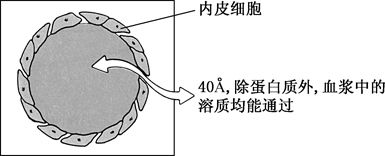
\includegraphics{./images/Image00034.jpg}
 \captionsetup{justification=centering}
 \caption{毛细血管壁吸收}
 \label{fig3-7}
  \end{figure} 

3.呼吸道吸收

即吸入给药(inhalation)。气体和挥发性药物(全麻药)及小颗粒(2μm):直接从肺泡吸收入血液,发挥全身作用。

肺泡表面积大(100~200m\textsuperscript{2}
),血流量大(肺毛细血管面积80m\textsuperscript{2}
),较大颗粒(10μm)的药物不被吸收,可在支气管和肺泡表面发挥局部作用(平喘药)。

4.皮肤和黏膜吸收(transdermal)

完整的皮肤吸收能力差,外用药物主要发挥局部作用。黏膜远较皮肤的吸收能力强。脂溶性药物可通过皮肤进入血液,如硝苯地平贴皮剂、硝酸甘油。

在过眼、鼻、喉、阴道等部位的局部用药主要是经黏膜吸收发挥局部作用,有时也可以发挥全身作用。

(二)影响吸收的因素

药物的理化性质、首过消除、吸收环境(如pH值、胃肠内容物、胃肠蠕动、胃肠血液循环等)。

\subsection{药物的分布及影响因素}

(一)分布

分布(distribution):药物吸收后随血液循环向组织、细胞间液和细胞内液转运的过程。是药物自血浆消除的方式之一。

药物的再分布(re-distribution):高脂溶性药物往往在用药早期最先分布在大脑中,因为大脑中枢神经组织脂溶性大、血流丰富,但随着时间的延长,这些药物又可随血液再向外周脂肪组织转移。

(二)影响分布的因素

1.与血浆蛋白的结合

药物可与血液中的清蛋白、β球蛋白、酸性白蛋白等结合。

\begin{figure}[!htbp]
 \centering
 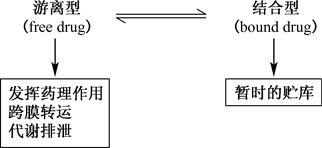
\includegraphics{./images/Image00035.jpg}
 \captionsetup{justification=centering}
 \caption{药物与血浆蛋白的结合}
 \label{fig3-8}
  \end{figure} 

与血浆蛋白结合的意义:

(1)游离型药物与药理作用强度密切相关,与血浆蛋白结合的药物无生物活性。

(2)结合型药物分子量增大,不跨膜转运,不被消除(代谢、排泄)。蛋白结合率高的药物,在体内消除较慢,作用维持时间较长。

(3)血浆蛋白量和质的改变可能影响高蛋白结合率药物的血药浓度。

(4)结合于同种血浆蛋白的药物可因竞争结合而使药浓升高,作用增强,不良反应及毒性增加。对血浆蛋白结合率高和游离浓度敏感的药物尤其要注意。如华法林(99%)与保太松、磺胺与甲苯磺丁脲。华法林单用时血浆蛋白结合率可能是95%,但当其他药物存在时,它的血浆蛋白结合率可能下降为90%,游离药物从5%增加到10%,增加了一倍,可能导致抗凝过度引起出血。

\begin{figure}[!htbp]
 \centering
 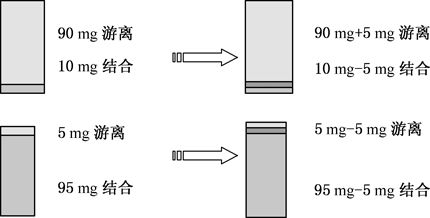
\includegraphics{./images/Image00036.jpg}
 \captionsetup{justification=centering}
 \caption{药物与血浆蛋白结合的意义}
 \label{fig3-9}
  \end{figure} 

与血浆蛋白结合率比较高的药物(>95%)有:甲状腺素、华法林、地西泮、呋塞米、肝素、丙咪嗪。

与血浆蛋白结合率为90%~95%的药物有:格列本脲、苯妥英、普萘洛尔、丙戊酸钠。

2.体内屏障

血脑屏障(blood brain
barrier):由血-脑、血-脑脊液及脑脊液-脑三种屏障组成,炎症等病理因素可以改变。

胎盘屏障(placental barrier)。

血眼屏障(blood eye barrier)。

3.其他

(1)局部器官血流量:血流丰富的器官,药物可迅速达到较高浓度。药物浓度在肝最高,肾、脑、心次之。皮肤、肌肉、脂肪、结缔组织血流量少,血药浓度依次降低。

(2)组织的亲合力:链霉素在内耳淋巴液,碘在甲状腺,强心甙在心脏。脂溶性的物质通常对脂肪组织有较高的亲和性。

(3)体液pH和药物的理化性质

在生理情况下细胞内液pH约为7.0,细胞外液pH约为7.48。弱酸性药物易自细胞内向细胞外转运,细胞外浓度高。弱碱性药物则相反,在细胞内浓度较高。

\subsection{药物的代谢}

1.药物代谢

药物代谢是指药物在体内发生的化学变化或称生物转化(bio-transformation)。

2.药物代谢时相和类型

Ⅰ相反应:氧化、还原、水解。

\begin{figure}[!htbp]
 \centering
 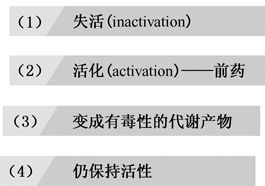
\includegraphics{./images/Image00037.jpg}
 \captionsetup{justification=centering}
 \caption{Ⅰ相反应的转归}
 \label{fig3-10}
  \end{figure} 

Ⅱ相反应:结合反应,如与葡萄糖醛酸、硫酸、醋酸、甘氨酸等结合反应。

3.药物代谢酶(drug metabolizing enzymes)

专一性酶:AChE,COMT,MAO等。

非专一性酶:约占56%。

肝脏微粒体混合功能酶系统(又称肝药酶),主要为细胞色素P450(CYP),是体内主要的药物代谢酶,大约有50%以上的药物由肝药酶代谢。

目前已知有18个基因家族、42个亚家族、57种酶,其中参与人体肝脏代谢的主要有CYP1、CYP2、CYP3及CYP4家族。人体已鉴定出12种CYP酶,其中CYP3A4(5)代谢的药物最多(约53%的药物),CYP2D6遗传氧化多态性最明显。

4.药物代谢酶的特性

(1)选择性低。

(2)变异性较大。

(3)活性有限,易饱和,有竞争性。

(4)易受外界因素诱导或抑制。

5.药物代谢酶的诱导与抑制

(1)酶诱导剂(enzyme
inducer):能够增强酶活性的药物。与耐受性、交叉耐受性、药物相互作用、个体差异等有关。如:

苯巴比妥合用双香豆素时,使双香豆疗效降低。

卡马西平与异烟肼合用,会导致异烟肼代谢产物增加,肝毒性增加。

利福平与避孕药合用,导致后者代谢加速,避孕失败、意外怀孕。

饮酒会导致扑热息痛(对乙酰氨基酚)肝毒性代谢产物增加,导致肝损害。

\begin{table}[htbp]
\centering
\caption{常用药酶诱导剂及受影响的药物}
\label{tabtab3-1}
\begin{tabular}{ll} 
    \toprule
    诱导剂 & 受影响的药物               \\ 
    \hline
    巴比妥类                     & 巴比妥类、氯丙嗪、香豆素类、地高辛、多西环素、苯妥英钠、可的松、奥美拉唑       \\
    苯妥英钠                     & 可的松、地高辛、硝苯地平、地西泮                           \\
    利福平                      & 香豆素类、地高辛、糖皮质激素类、美沙酮、美托洛尔、口服避孕药、普茶洛尔、奥美拉唑  \\
    \bottomrule
    \end{tabular}
\end{table}

(2)酶抑制剂(enzyme inhibiter):能够减弱酶活性的药物。

常见的肝药酶抑制剂有氯霉素、丙戊酸盐、磺胺类药、保泰松、胺碘酮、奥美拉唑等。

\begin{table}
\centering
\caption{常用药酶抑制剂及受影响的药物}
\label{tab3-2}
\begin{tabular}{ll} 
\toprule
\begin{tabular}[c]{@{}l@{}}抑制剂\\\end{tabular} & 受影响的药物            \\
    \midrule
氯霉素异烟肼                                        & 双香豆素、丙磺舒、甲苯磺丁脲    \\
西味替丁                                          & 可的松、地高辛、硝苯地平、地西泮  \\
\bottomrule
\end{tabular}
\end{table}

保泰松对肝药酶活性的改变依合用药物种类不同而异:对可的松、地高辛等药是酶诱导剂,对甲苯磺丁脲、苯妥英钠则是酶抑制剂。可能是由于保泰松对不同类型的CYP分别起诱导和抑制作用所致。

特非那定(抗组胺药)、阿司咪唑(息司敏)易受多种肝药酶抑制剂影响,导致心脏毒性大增而停用。苄普地尔(mibefradil)因强肝药酶抑制作用而停止上市。

\subsection{药物的排泄}

排泄(excretion)是指药物及其代谢物经机体的排泄器官或分泌器官排出体外的过程。

\begin{figure}[!htbp]
 \centering
 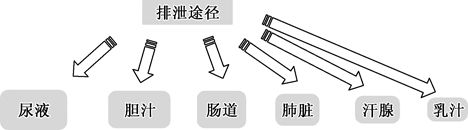
\includegraphics{./images/Image00040.jpg}
 \captionsetup{justification=centering}
 \caption{药物排泄的途径}
 \label{fig3-11}
  \end{figure} 

1.肾排泄

肾是主要的排泄器官。

\begin{figure}[!htbp]
 \centering
 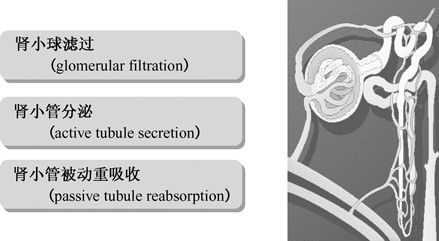
\includegraphics{./images/Image00041.jpg}
 \captionsetup{justification=centering}
 \caption{药物经肾排泄}
 \label{fig3-12}
  \end{figure} 

\begin{table}[htbp]
\centering
\caption{经肾排泄的药物}
\label{tab3-3}
\begin{tabular}{ll} 
\toprule
弱酸性药物 & 弱碱性药物  \\
\midrule
阿司匹林                                            & 吗啡     \\
头孢噻啶                                            & 哌替啶    \\
呋塞米                                             & 氨苯蝶啶   \\
青霉素                                             & 多巴胺    \\
噻嗪类利尿药                                          &        \\
丙磺舒                                             &        \\
\bottomrule
\end{tabular}
\end{table}

(1)肾小管分泌是主动转运过程:载体分为酸性药物载体和碱性药物载体两类,同类药物之间会发生竞争。

一些由肾小管主动分泌排泄的弱酸性药物和弱碱性药物,如丙磺舒,可竞争分泌机制,影响青霉素和头孢菌素的作用强度及时间。

呋塞米、水杨酸盐、保泰松、别黄嘌呤可与尿酸竞争分泌机制,使尿酸排泄减少,体内尿酸增加,加重痛风。

(2)肾小管重吸收:主要通过异化扩散方式重吸收。

尿液pH值对药物排泄的影响较大。尿液pH影响尿液的重吸收和最终排泄。

意义:改变尿液pH值可以改变药物的排泄速度,用于药物中毒的解毒或增强疗效。

弱酸性药物(如巴比妥、阿司匹林)在碱性尿液中解离多,重吸收少,排泄快,因此,酸性药物中毒时,可以用小苏打、乙酰唑胺和多食蔬菜等方式碱化尿液,加速药物排泄。

弱碱性药物(如吗啡、阿托品、交感胺、抗组胺药)则相反,在酸性尿液中解离多,重吸收少,排泄快,因此,碱性药物中毒时,可以用氯化铵、汞利尿剂等方式酸化尿液,加速药物排泄。

\begin{figure}[!htbp]
 \centering
 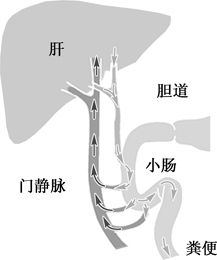
\includegraphics{./images/Image00043.jpg}
 \captionsetup{justification=centering}
 \caption{药物的肝肠循环}
 \label{fig3-13}
  \end{figure} 

2.胆汁排泄

(1)胆汁浓度高:氨苄西林、头孢哌酮、利福平、红霉素等主要经过胆汁排泄,故可用于敏感菌的肝胆道感染。

(2)分子量大于300的药物(多为结合型药物)易于自胆汁分泌,随胆汁排进十二指肠的结体型药物在肠中经分解为小分子药物后再吸收,形成肝-肠循环(hepato-enteral
circulation),使药物作用时间延长。

(3)强心苷类中毒的解救:同时服用消胆胺可阻断肝肠循环,加速药物排泄。

3.其他排泄途径

(1)肠道:碱性药物(吗啡、阿托品等)在高血药浓度时从血浆以被动扩散的方式从胃肠黏膜排泄,及时洗胃可以加快排泄,否则排到肠腔可再次吸收。

(2)母乳:偏酸性,pH约6.6,碱性药物在母乳中浓度高(如吗啡、阿托品、红霉素、乙醇)。

(3)肺:吸入性药物的主要排泄途径。

(4)汗腺、唾液腺、泪腺。

(5)头发:含量少,但有法医学意义。

\section{消除速率过程}

\subsection{药物浓度-时间曲线}

用药后,药物在血浆的浓度(量)随着时间(时)的推移而发生变化,这种变化可以浓度(或对数浓度)为纵坐标和以时间为横坐标作图,即为时-量曲线(time-concentration
curve)。

\begin{figure}[!htbp]
 \centering
 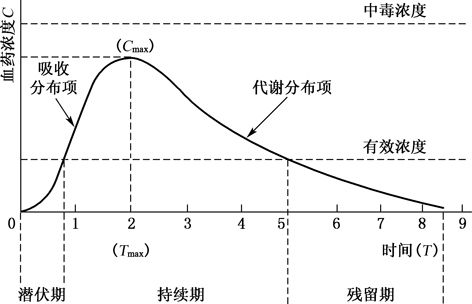
\includegraphics{./images/Image00044.jpg}
 \captionsetup{justification=centering}
 \caption{时-量曲线}
 \label{fig3-14}
  \end{figure} 

\subsection{药物消除速率}

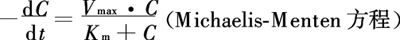
\includegraphics{./images/Image00045.jpg}

当K\textsubscript{m} ≫C时,则

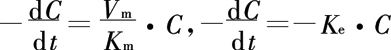
\includegraphics{./images/Image00046.jpg} ,称为一级消除动力学(first
order elimination kinetics)。

当C≫K\textsubscript{m} 时,则

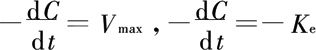
\includegraphics{./images/Image00047.jpg} ,称为零级消除动力学(zero
order elimination kinetics)。

\subsection{药物消除方式}

一级动力学消除:单位时间内消除药物的百分率不变,与血药浓度成正比,也称定比消除(恒比消除)。例如:-50%/12h。

\begin{figure}[!htbp]
 \centering
 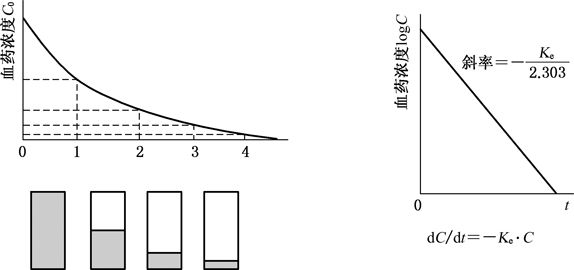
\includegraphics{./images/Image00048.jpg}
 \captionsetup{justification=centering}
 \caption{一级动力学消除}
 \label{fig3-15}
  \end{figure} 

零级动力学消除:指血药浓度按恒定速度进行消除,与血药浓度无关,也称为定量消除(恒量消除)。例如:-5g/12h。

\begin{table}[htbp]
\centering
\caption{药物消除的方式}
\label{tab3-4}
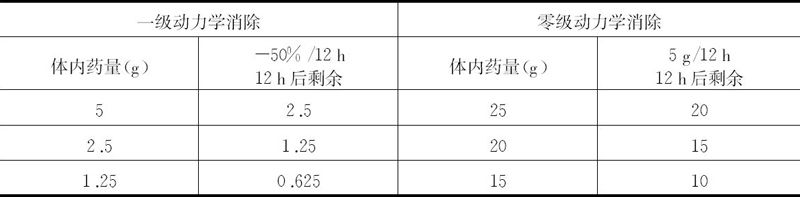
\includegraphics{./images/Image00049.jpg}
\end{table}

\begin{figure}[!htbp]
 \centering
 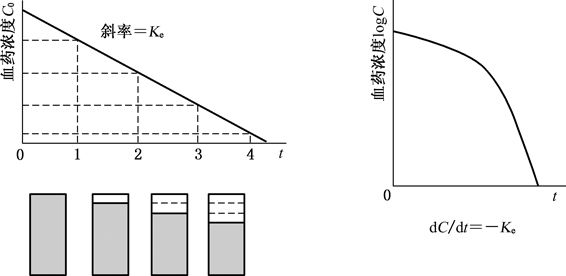
\includegraphics{./images/Image00050.jpg}
 \captionsetup{justification=centering}
 \caption{零级动力学消除}
 \label{fig3-16}
  \end{figure} 

半衰期(half-life, t\textsubscript{1/2}
):一般指血浆半衰期,即血浆药物浓度下降一半所需要的时间。

一级动力学消除半衰期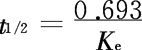
\includegraphics{./images/Image00051.jpg}

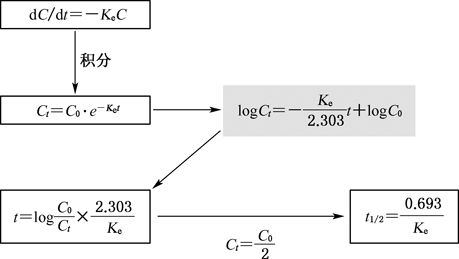
\includegraphics{./images/Image00052.jpg}

零级动力学消除半衰期: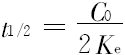
\includegraphics{./images/Image00053.jpg}

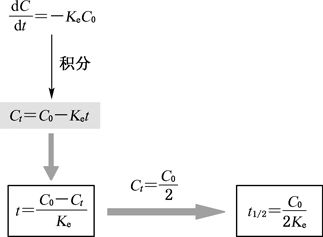
\includegraphics{./images/Image00054.jpg}

\begin{table}[htbp]
\centering
\caption{一级动力学消除与零级动力学消除的区别}
\label{tab3-5}
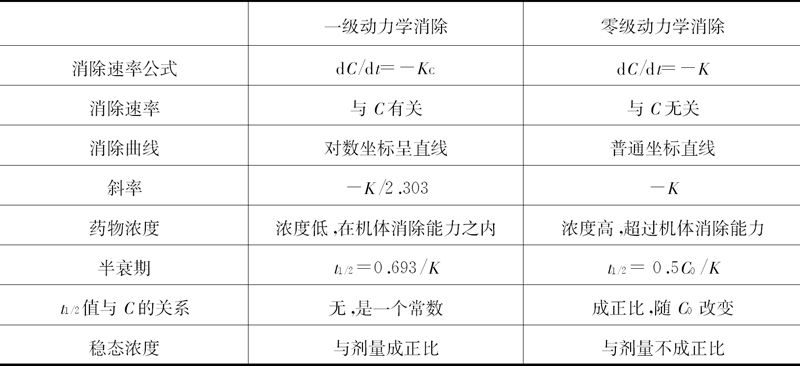
\includegraphics{./images/Image00055.jpg}
\end{table}

\subsection{房室模型}

1.根据药代动力学特性,将房室模型(compartment
model)分为一房室模型、二房室模型和多房室模型

房室是便于分析的抽象概念,只要机体某些部位接受药物和消除药物的速率常数相似,不管解剖位置和生理功能都归纳为一个单位,即一个房室。

\begin{figure}[!htbp]
 \centering
 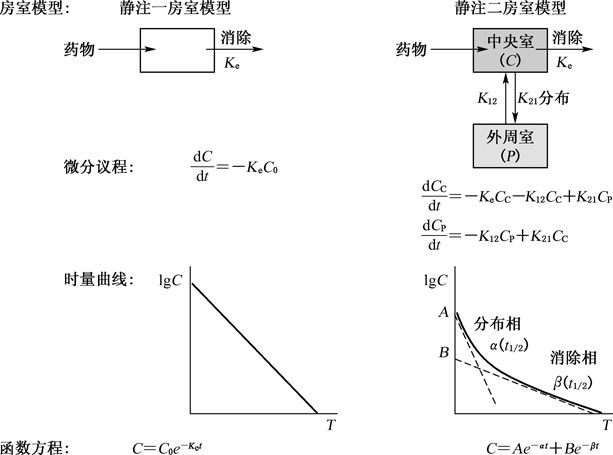
\includegraphics{./images/Image00056.jpg}
 \captionsetup{justification=centering}
 \caption{静脉注射给药一房室和二房室模型示意图}
 \label{fig3-17}
  \end{figure} 

2.其他模型

(1)生理药物动力学模型(physiological-pharmacological
model):根据生理解剖(每个器官看成一个房室,器官大小、组织血流量),生化(酶活性)、药物热力学(脂溶性,解离度)等参数代入相应的模型,用计算机可以计算每个组织器官的参数。

(2)药动-药效学组合模型(combined pharmacokinetic-pharmacodynamic
model)、血药浓度与药物效应的时间关系(滞后性):血浓度-时间-效应关系。

(3)统计矩(statistical
model):通过实验得到AUC数据来计算三个统计矩总量零阶矩(AUC)、一阶矩(MRT:mean
residence time平均驻留时间)、二阶矩(VRT:variance of mean residence
time差异)、表观半衰期、表观清除率、生物利用度、平均稳态浓度、达稳时间、平均吸收时间、平均溶解时间、平均崩解时间等动力学参数概念。

\subsection{药动学参数计算及意义}

1.峰浓度

\begin{figure}[!htbp]
 \centering
 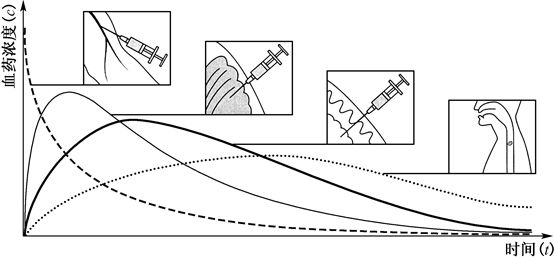
\includegraphics{./images/Image00057.jpg}
 \captionsetup{justification=centering}
 \caption{不同给药途径的峰浓度}
 \label{fig3-18}
  \end{figure} 

2.曲线下面积

曲线下面积(area under curve,
AUC):指药物浓度-时间曲线下面积,单位为mg/(h·L)或ng/(min·ml)。AUC可用积分法或梯形法测得,反映进入体循环的药量,常用于估算C\textsubscript{L}
,独立于房室模型的指标。

\begin{figure}[!htbp]
 \centering
 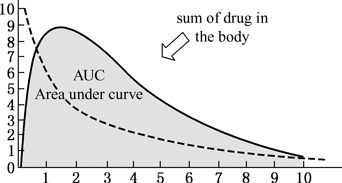
\includegraphics{./images/Image00058.jpg}
 \captionsetup{justification=centering}
 \caption{AUC}
 \label{fig3-19}
  \end{figure} 

\begin{figure}[!htbp]
 \centering
 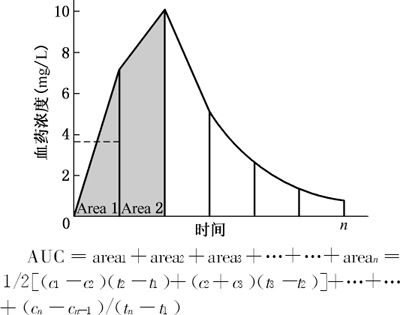
\includegraphics{./images/Image00059.jpg}
 \captionsetup{justification=centering}
 \caption{矩形面积计算法}
 \label{fig3-20}
  \end{figure} 

积分法则AUC

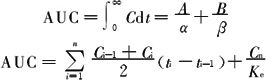
\includegraphics{./images/Image00060.jpg}

AUC=C\textsubscript{0} /K 一次静脉注射iv

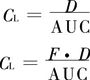
\includegraphics{./images/Image00061.jpg}

3.生物利用度

生物利用度(bioavailability,
F):指血管外给药后被吸收进入体循环的药物相对分量和速度,是评价两个药物是否具有生物等效性的重要参数。常用的评价指标是在同一受试者比较两个制剂的AUC、T\textsubscript{max}
、C\textsubscript{max} 。

生物等效性:指一种药物的相同或不同制剂在相同的试验条件下,给以相同的剂量,其活性成分吸收的程度和速度是否接近或相同。

生物利用度 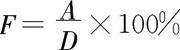
\includegraphics{./images/Image00062.jpg}

绝对生物利用度 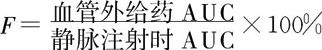
\includegraphics{./images/Image00063.jpg}

相对生物利用度 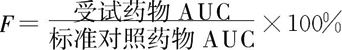
\includegraphics{./images/Image00064.jpg}

AUC主要反应吸收程度。吸收速度T\textsubscript{max} 、C\textsubscript{max}
影响初始浓度,也同样影响疗效。

\begin{figure}[!htbp]
 \centering
 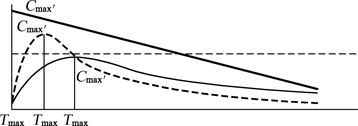
\includegraphics{./images/Image00065.jpg}
 \captionsetup{justification=centering}
 \caption{C\textsubscript{max} 与T\textsubscript{max}}
 \label{fig3-21}
  \end{figure} 

4.表观分布容积

表观分布容积(apparent volume of distribution, V\textsubscript{d}
)指药物在体内分布达到平衡时,按测得的血药浓度(C)计算该药应占有的容积(V\textsubscript{d}
或V)。以L或L/kg表示。表观分布容积并非药物在体内真正占有的体液容积,故称“表观”分布容积。

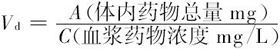
\includegraphics{./images/Image00066.jpg}

V\textsubscript{d} 意义:

(1)V\textsubscript{d}
值代表药物在体内分布范围的广窄,但超过机体容积多倍的V\textsubscript{d}
值则提示药物在体内某些器官组织高浓度积蓄。

甘露醇(mannitol)V\textsubscript{d} ≈0.06;静注后分布于血浆。

链霉素(streptomycin)V\textsubscript{d} =0.25;分布于细胞外液。

异烟肼(isoniazid)V\textsubscript{d} =0.67;分布于细胞的外液和内液。

利福平(rifampin)V\textsubscript{d}
=0.97;穿透力强,可分布达全身体液和脂溶性物质。

氯喹(chloroquine)V\textsubscript{d}
=115,是机体容积的百倍以上,在肝、肺和脾脏高浓度积聚。

(2)分布容积越小药物排泄越快,体内存留时间越短;分布容积越大药物排泄越慢,体内存留时间越长。

(3)计算给药量A=C·V\textsubscript{d} 。

5.消除速率常数(K\textsubscript{e} )

指单位时间内清除药物的百分数,是各种途径消除药物的总和,通常是一个常数。如0.18/h,表示每小时消除18%。

消除速率常数 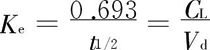
\includegraphics{./images/Image00067.jpg}

6.半衰期(half-life, t\textsubscript{1/2} )

通常指血浆半衰期,即血浆药物浓度下降一半所需要的时间。

一级动力学消除的药物:

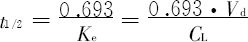
\includegraphics{./images/Image00068.jpg}

零级动力学消除的药物:

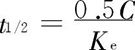
\includegraphics{./images/Image00069.jpg}

半衰期(t\textsubscript{1/2} )的意义:

(1)反映药物消除快慢,间接反映肝肾功能清除率。

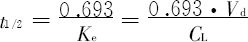
\includegraphics{./images/Image00068.jpg}

(2)根据t\textsubscript{1/2}
确定给药间隔,一般略等于或接近该药的t\textsubscript{1/2} 。

(3)根据半衰期分类:超短效(<1h),短效(1~4h),中效(4~8h),长效(8~24h),超长效(>24h)。

(4)预测连续给药或改变给药速度后达到稳态血药C\textsubscript{ss}
的时间,或预测停药后血药基本消除的时间。

每隔一个t\textsubscript{1/2} 给药C\textsubscript{0}
,药物在体内累积量C\textsubscript{t} =C\textsubscript{0}
[1-(1/2)\textsuperscript{n}
],需经过该药的4~5个t\textsubscript{1/2} 才能达到96.5%。

每隔一个t\textsubscript{1/2} 药物在体内消除的量C\textsubscript{t}
=C\textsubscript{0} (1/2)\textsuperscript{n}
,停药后经过4~5个t\textsubscript{1/2} 后,血药浓度约下降96%。

\begin{table}[htbp]
\centering
\caption{半衰期与体内药物}
\label{tab3-6}
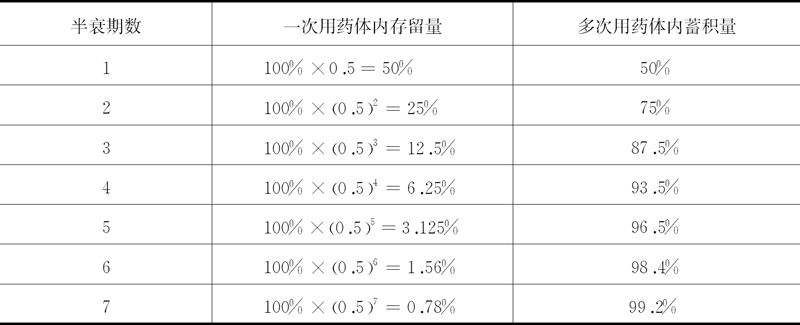
\includegraphics{./images/Image00070.jpg}
\end{table}

7.清除率

消除率(clearance)指机体清除的药物总量与其血浆浓度的比值,即单位时间内被清除药物表观容积数。


\includegraphics{./images/Image00071.jpg}
 单位:L/(h·kg)或ml/(min·kg)

当以恒定的速度给药时,如果达到稳态浓度C\textsubscript{ss}
,此时给药速率等于清除率。

单次给药时: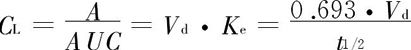
\includegraphics{./images/Image00072.jpg}

多次给药时: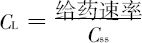
\includegraphics{./images/Image00073.jpg}

C\textsubscript{L总} =C\textsubscript{L肾脏} +C\textsubscript{L肝脏}
+C\textsubscript{L其他} ,反映肝肾功能。

R=C\textsubscript{L} ·C\textsubscript{ss}

\begin{table}[htbp]
\centering
\caption{主要药代学参数之间的关系}
\label{tab3-7}
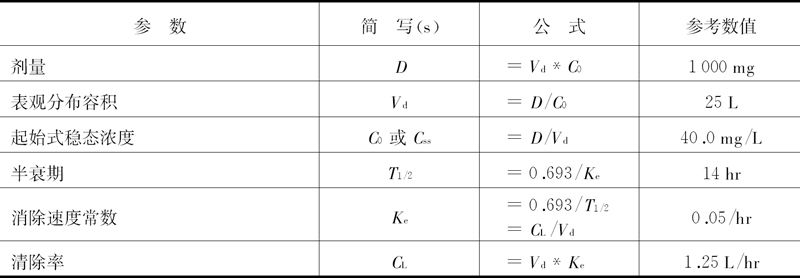
\includegraphics{./images/Image00074.jpg}
\end{table}

\subsection{多次给药}

(一)稳态浓度

(1)按照一级消除动力学的规律,连续给药5个t\textsubscript{1/2}
血浆中药物浓度达到稳态浓度(steady-state concentration,
C\textsubscript{ss} ),稳态浓度也称坪值(plateau)。

(2)达到C\textsubscript{ss} 时,给药速度与消除速度相等。

(3)C\textsubscript{ss} 可用单次给药的AUC[(g·h)/L]计算:

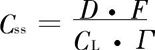
\includegraphics{./images/Image00075.jpg}

D:给药剂量;F:生物利用度;C\textsubscript{L} :清除率;Г:给药间隔。

\begin{figure}[!htbp]
 \centering
 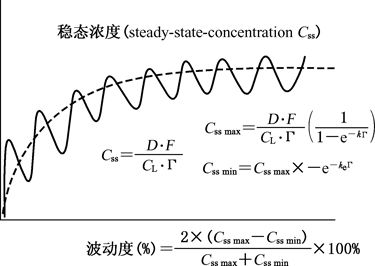
\includegraphics{./images/Image00076.jpg}
 \captionsetup{justification=centering}
 \caption{多次给药后的时量曲线}
 \label{fig3-22}
  \end{figure} 

累积因子R:多次给药后药物在体内的累积程度。

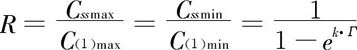
\includegraphics{./images/Image00077.jpg}

当Γ=t\textsubscript{1/2} ,R=1.44。

当Γ<t\textsubscript{1/2} ,药物大于1.44的倍数累积。

当Γ>t\textsubscript{1/2} ,药物小于1.44的倍数累积。

(二)临床多次给药方法

1.维持量

一般需要4~5个半衰期(分次给药或持续静脉滴注)达到稳态浓度C\textsubscript{ss}
,此时的给药量等于消除量,称为维持量。剂量与C\textsubscript{ss}
成正比,增加剂量可增加C\textsubscript{ss} ,但达到C\textsubscript{ss}
的时间不变。

维持量(maintenance dosage)

\includegraphics{./images/Image00078.jpg}

2.负荷量(loading dosage)

为使稳态治疗浓度提前产生而加大的首次剂量,称为负荷量。

\includegraphics{./images/Image00079.jpg}

如果D\textsubscript{m} =1g,Γ=t\textsubscript{1/2} =4h

\includegraphics{./images/Image00080.jpg}

为使血药浓度迅速达到C\textsubscript{ss}
,在第一半衰期内给予2倍的维持量,即负荷量D\textsubscript{L}
=2D\textsubscript{m} 。

持续静脉滴注时,在第一个半衰期内将原维持量增加1.44倍。C\textsubscript{ss}
=1.44R\textsubscript{A} ·/V\textsubscript{d}
,可使血药浓度迅速达到C\textsubscript{ss} 。

\section*{大纲要求}

1.掌握一级消除动力学及零级消除动力学的特点。

2.掌握首过消除、肝肠循环、房室模型、药代动力学基本参数曲线下面积、生物利用度、生物等效性、表观分布容积、半衰期、清除率、稳态浓度、负荷量的概念及意义。

